\section*{3}
In this pictures we can see the moralized edge(red) and the one for
triangulation(green). As the onle 2 nodes with same children are B1 and 
B4, are the only edge that we add in the moralized phase. The green edge
is added in the triangulation phase as the B1,B2,B3,B4 are the only clique.
\begin{figure}[ht]
  \begin{subfigure}[b]{0.5\linewidth}
    \centering
    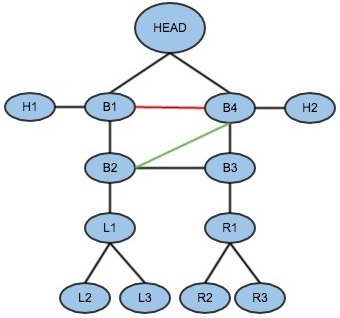
\includegraphics[width=0.75\linewidth]{figures/ml5.jpg}
    \caption{Moralized/Triangulated graph}
    \vspace{4ex}
  \end{subfigure}%%
  \begin{subfigure}[b]{0.5\linewidth}
    \centering
    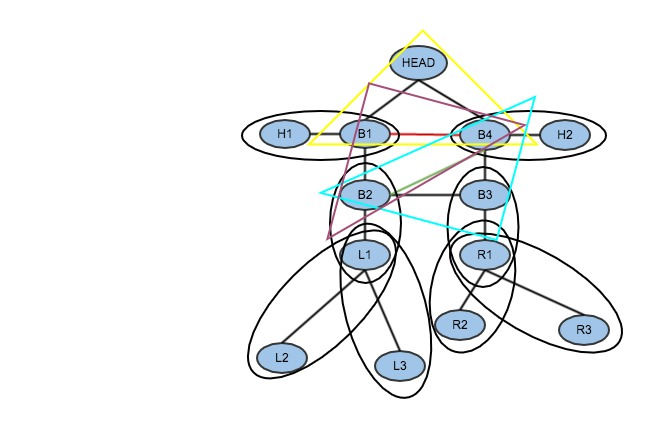
\includegraphics[width=0.75\linewidth]{figures/ml5triang.jpg}
    \caption{Clique graph}
    \vspace{4ex}
  \end{subfigure}
\end{figure}
\clearpage
\begin{figure}[ht]
    \centering
    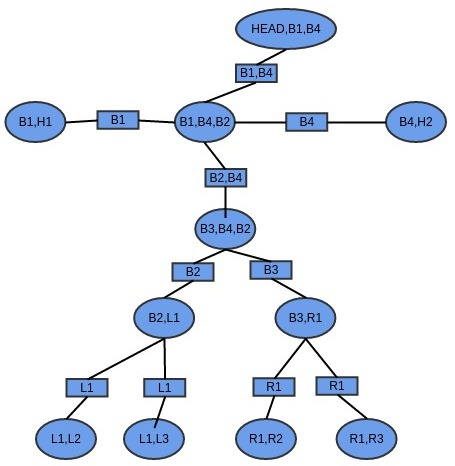
\includegraphics[width=0.75\textwidth]{figures/ml5JT.jpg}
    \caption{Junction Tree}
\end{figure}
